\documentclass{beamer}
\usetheme{ucl}

%Path relative to the main .tex file 
\graphicspath{ {./images/} }
\usepackage[style=authoryear-ibid,backend=biber,doi=false,isbn=false,url=false]{biblatex}
\addbibresource{references.bib}

\usepackage[export]{adjustbox}
% \usepackage[noindent,UTF8]{ctexcap}

%%% Increase the height of the banner: the argument is a scale factor >=1.0
% \setbeamertemplate{banner}[ucl][1.5]

%%% Change the colour of the main banner
%%% The background should be one of the UCL colours (except pink or white):
%%%   black,darkpurple,darkred,darkblue,darkgreen,darkbrown,richred,midred,
%%%   navyblue,midgreen,darkgrey,orange,brightblue,brightgreen,lightgrey,
%%%   lightpurple,yellow,lightblue,lightgreen,stone
% \setbeamercolor{banner}{bg=darkpurple}
% \setbeamercolor{banner}{bg=yellow,fg=black}

%%% Add a stripe behind the banner
% \setbeamercolor{banner stripe}{bg=brightblue,fg=black}

%%% The main structural elements
% \setbeamercolor{structure}{fg=black}

%% Author/Title/Date and slide number in the footline
\setbeamertemplate{footline}[author title date]

% \setbeamertemplate{footline}[page number]

%%% Puts the section/subsection in the headline
% \setbeamertemplate{headline}[section]

%%% Puts a navigation bar on top of the banner
%%% For this to work correctly, the each \section command needs to be
%%% followed by a \subsection. Requires one extra compile.
% \setbeamertemplate{headline}[miniframes]
%%% Accepts an optional argument determining the width
% \setbeamertemplate{headline}[miniframes][0.3\paperwidth]


%%% Puts the frame title in the banner
%%% Won't work correctly with the above headline templates
% \useoutertheme{ucltitlebanner}
%%% Similar to above, but smaller (and puts subtitle on same line as title)
% \useoutertheme[small]{ucltitlebanner}

%%% Gives block elements (theorems, examples) a border
% \useinnertheme{blockborder}
%%% Sets the body of block elements to be clear
% \setbeamercolor{block body}{bg=white,fg=black}

% %% Include CSML logo on title slide
% \titlegraphic{\includegraphics[width=0.16\paperwidth]{csml_logo}}

%%% Include CSML logo in bottom right corner of all slides
% \logo{\includegraphics[width=0.12\paperwidth]{csml_logo}}

%%% Set a background colour
% \setbeamercolor{background canvas}{bg=lightgrey}

%%% Set a background image
%%% Some sample images are available from the UCL image store:
%%%   https://www.imagestore.ucl.ac.uk/home/start
% \setbeamertemplate{background canvas}{%
%   \includegraphics[width=\paperwidth]{imagename}}



%%%%%% Some other settings that can make things look nicer
%%% Set a smaller indent for description environment
\setbeamersize{description width=2em}
%%% Remove nav symbols (and shift any logo down to corner)
% \setbeamertemplate{navigation symbols}{\vspace{-2ex}}
% \setbeamertemplate{footline}[page number]

\title[OSRM]{Open Street Routing Machine: an introduction}
% \author[Auth. 1 \and Auth.2 \and Auth.3 \and Auth.4]{Huanfa Chen \and Yanjia Cao \and Lingru Feng \and Qunshan Zhao}
% \institute[UCL]{%
%   Centre for Advanced Spatial Analysis, UCL \\ %
% %   University College London
% }
\author[Chen]{Huanfa Chen \inst{1} }
\institute[CASA]{\inst{1} Centre for Advanced Spatial Analysis, UCL \and %
%                       \inst{2} Department of Geography, Hong Kong University \and %
%                       \inst{3} Urban Big Data Centre, University of Glasgow
                      }
\date{15 June 2022}
% \setbeamertemplate{footline}[frame number]

\begin{document}

\begin{frame}
  \titlepage%
\end{frame}

% Outline frame
\begin{frame}{Outline}
    \tableofcontents[hideallsubsections]
\end{frame}

% Current section
\AtBeginSection[ ]
{
\begin{frame}{Outline}
    \tableofcontents[currentsection,hideallsubsections,subsubsectionstyle=hide]
\end{frame}
}

\section{Introduction}
\begin{frame}{Seminar outline}
\begin{enumerate}
\item 06/16: 路线规划的开源软件及应用(第一部分:软件介绍)
\item 06/23: 路线规划的开源软件及应用(第二部分:实践操作)
\item 06/30: 城市设施选址问题(第一部分:模型介绍)
\item 07/07: 城市设施选址问题(第二部分:开源软件)
\item 07/14: 城市设施选址问题(第三部分:案例分析)
\item 07/21: 选址-路线规划问题:无人机基站选址的案例
\end{enumerate}
\end{frame}


% Presentation structure
\section{Questions on routing}
\begin{frame}
\frametitle{Using a paper map for routing?}
\begin{columns}[T]
%     \begin{column}{.5\textwidth}
%   \end{column}
    \begin{column}{\textwidth}
    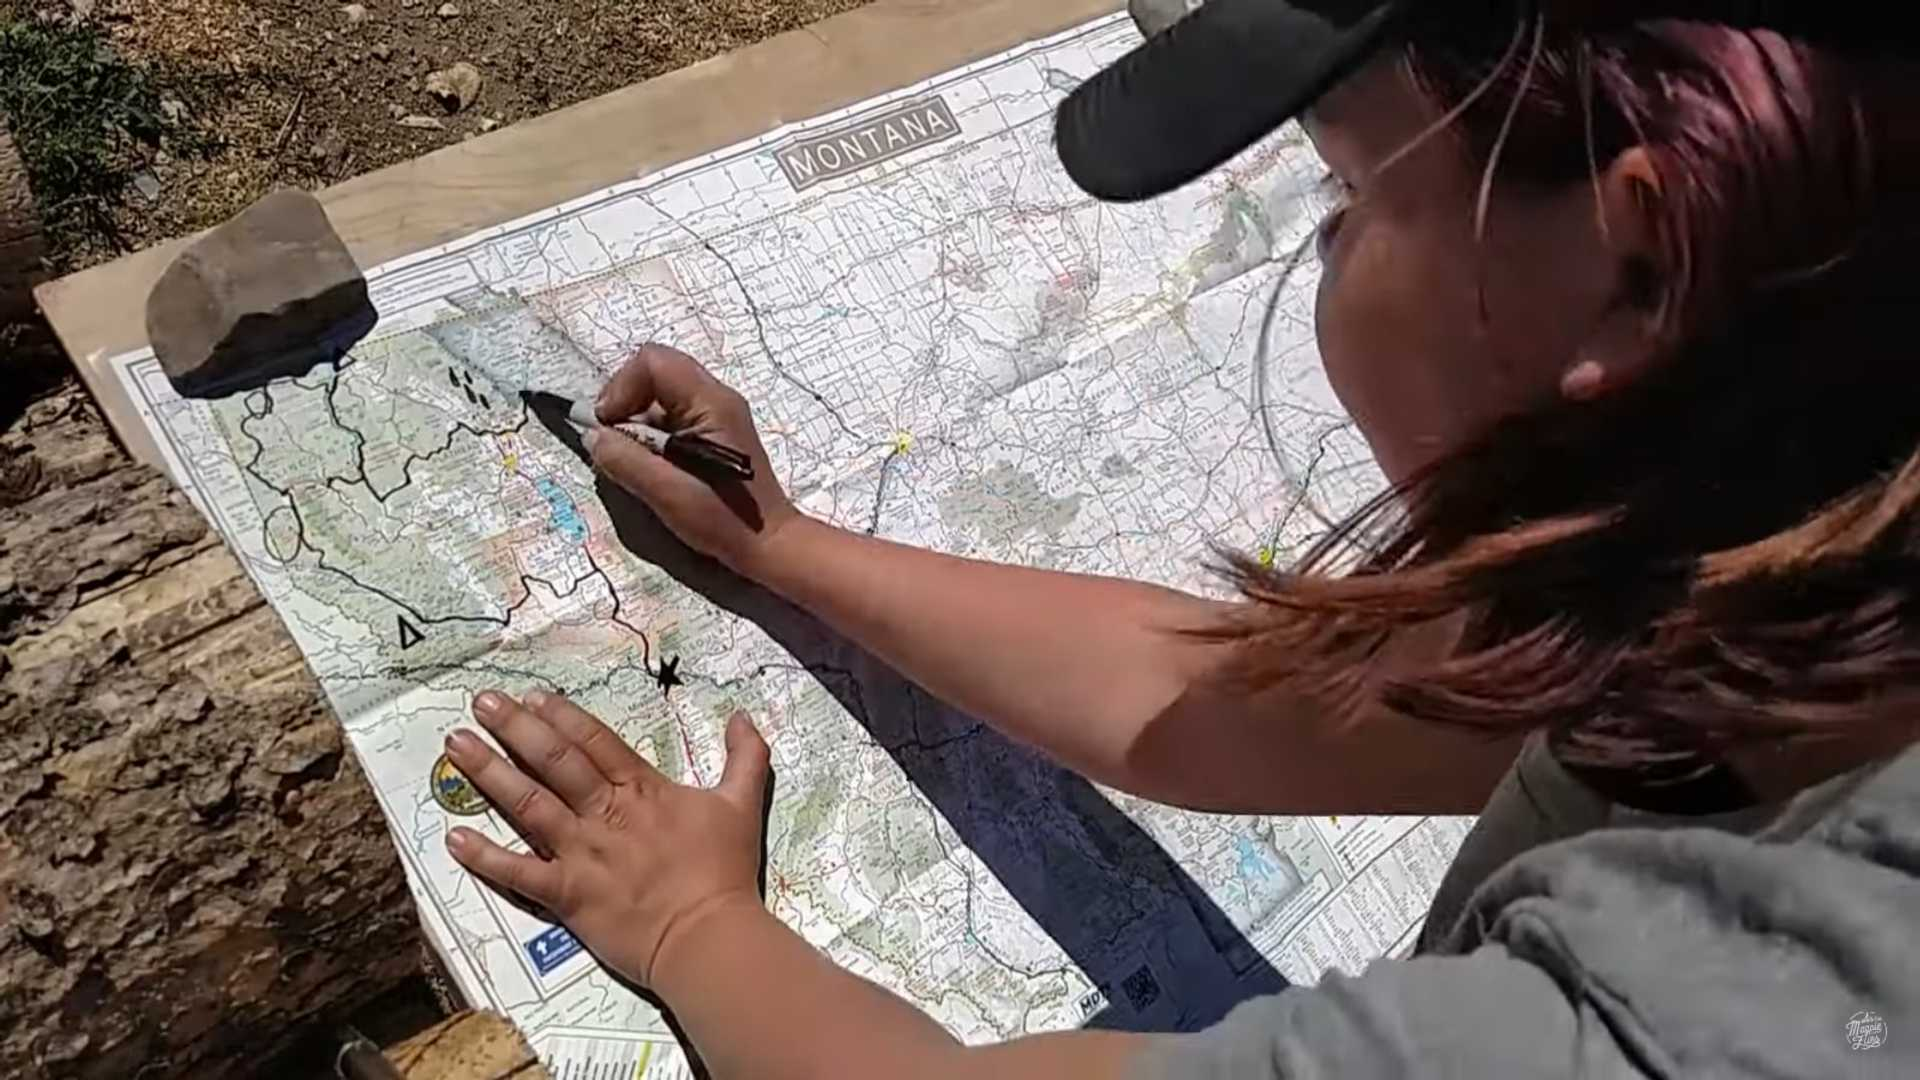
\includegraphics[max size={\textwidth}{\textheight}]{images/route-planning-on-paper-map.jpg}
    \end{column}
  \end{columns}
%   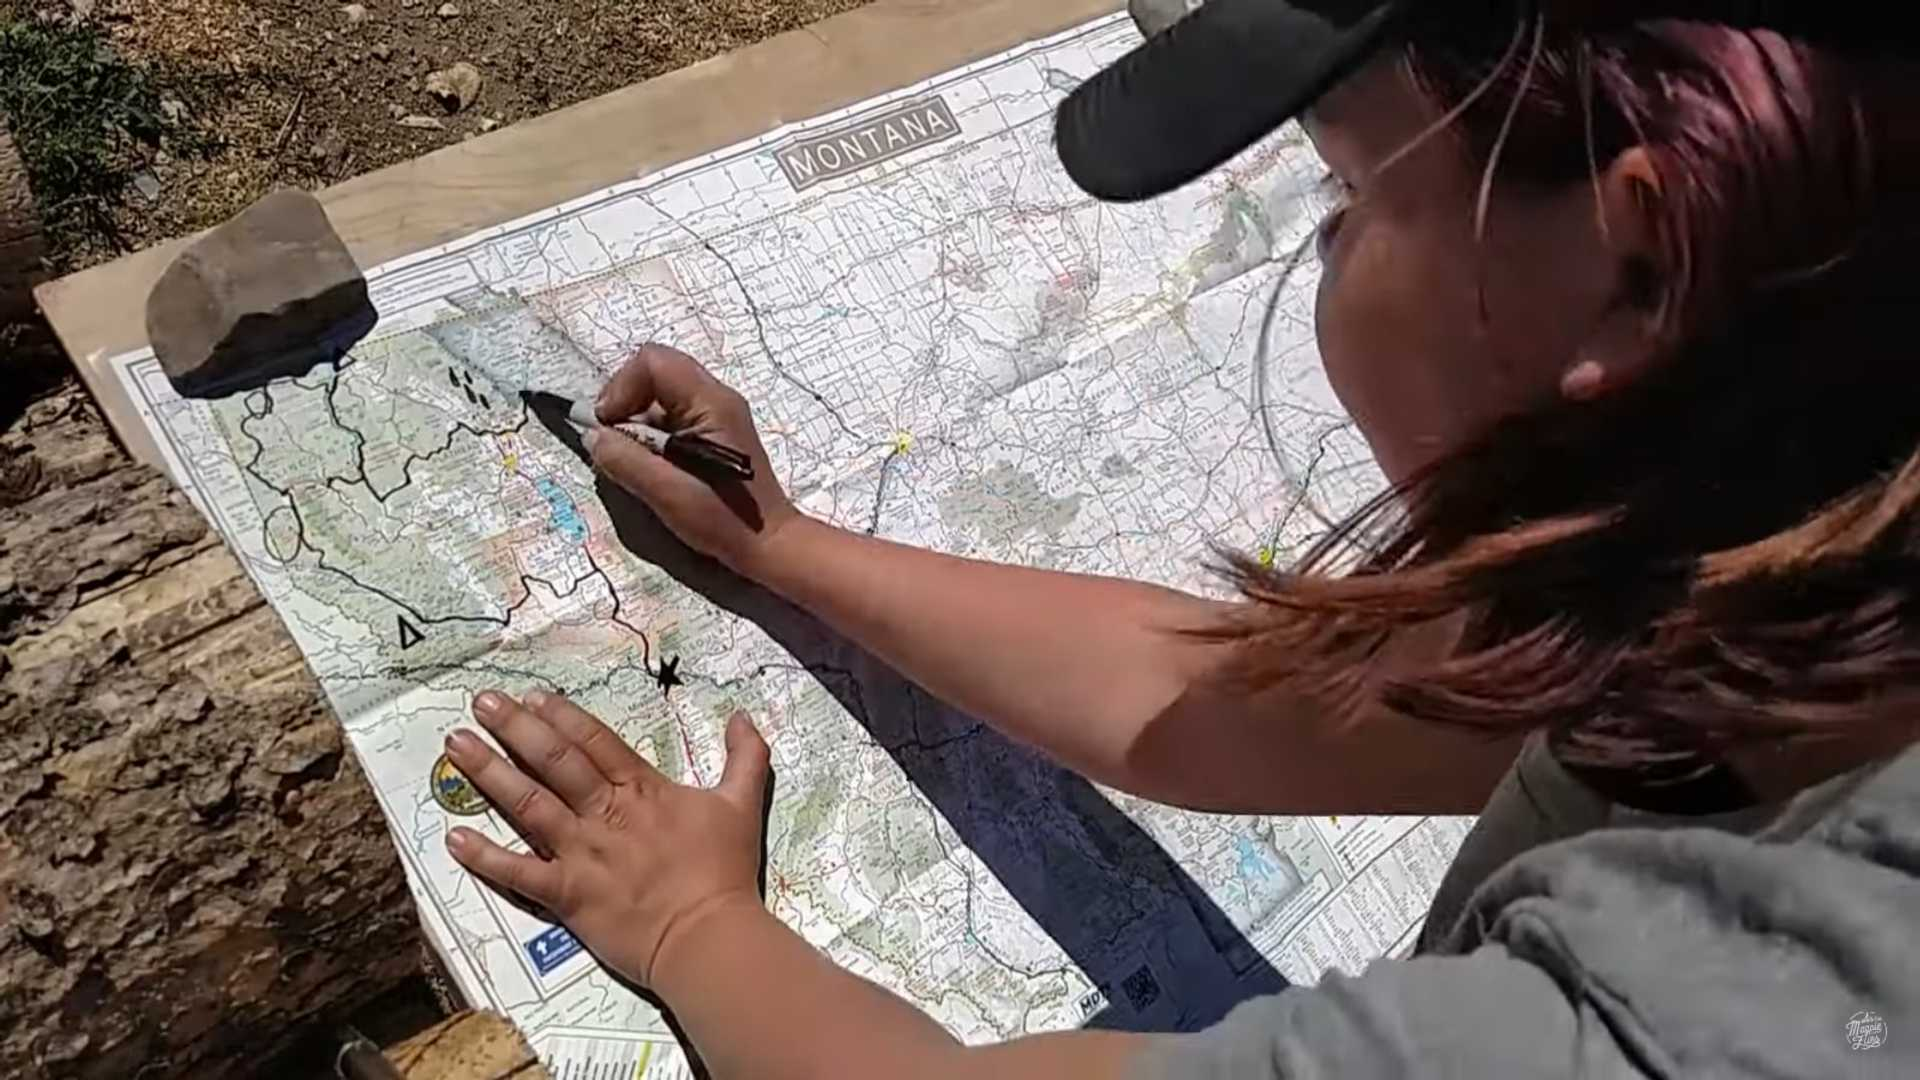
\includegraphics[width=\textwidth]{images/route-planning-on-paper-map.jpg}
\end{frame}
\begin{frame}
\frametitle{Questions on routing}
  \begin{itemize}
  \item Have you used routing software (e.g. Baidu Map, Gaode Map)?
  \item Are these software free?
  \item What are the problems of these software?
  \end{itemize}
\end{frame}
\section{Introduction to OSRM}

\begin{frame}
\frametitle{Open Street Routing Machine}
  \begin{itemize}
  \item An open-source modern C++ routing engine for shortest paths in road networks
  \item An open-source alternative to Google Map, Gaode Map (Amap), Baidu Map, et al.
  \item The network data is based on OpenStreetMap.
  \item The server can be deployed in an off-line environment without Internet
  \item Supporting driving, bike, foot (but not public transport)
  \end{itemize}
\end{frame}

\begin{frame}
\frametitle{Why we need OSRM (given that Google/Gaode/Baidu Maps are free and fast)?}
  \begin{itemize}
  \item \textbf{Not free for large-scale queries}: when you have millions of queries (0.04 USD per query)
  \item \textbf{Not secure for high-security projects}: you need to visit Internet; anyone may be forbidden to use these APIs (up to company decisions)
  \item \textbf{Not customisable} (if you want to change the road network or simulate the effect of new infrastructures)
%   \item The server can be deployed in an off-line environment without Internet
%   \item Supporting driving, bike, foot (but not public transport)
  \end{itemize}
\end{frame}

\begin{frame}
\frametitle{Why we need road network distance (many geography/transport papers using Euclidean distance)}
  \begin{columns}[T]
%     \begin{column}{.5\textwidth}
%   \end{column}
    \begin{column}{0.6\textwidth}
    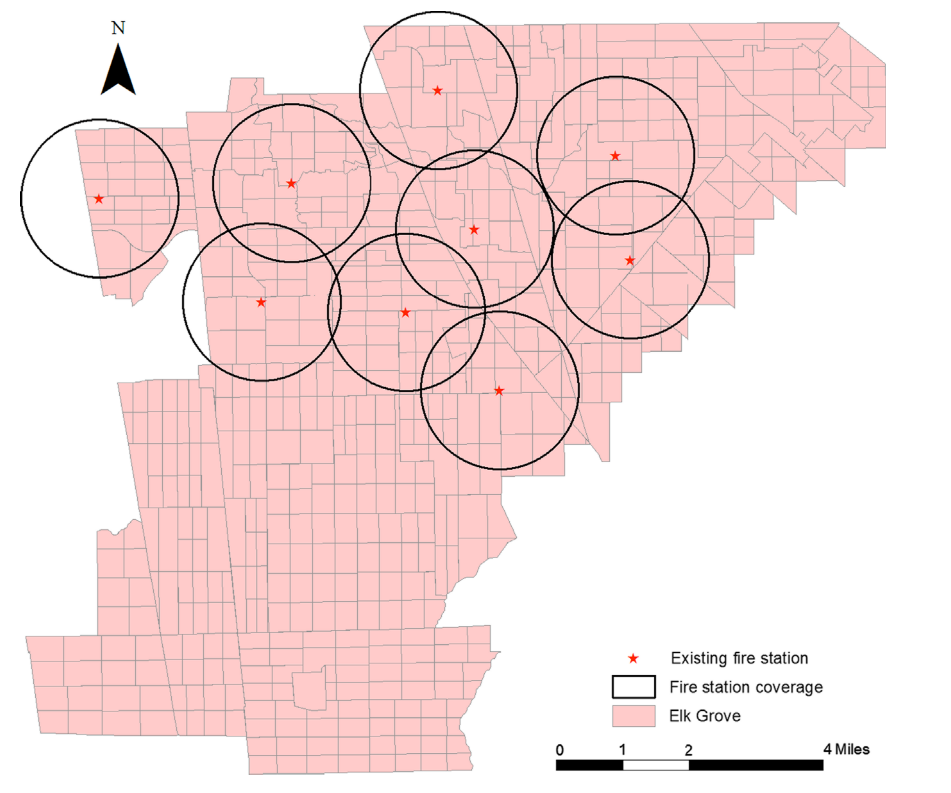
\includegraphics[max size={\textwidth}{\textheight}]{images/Example_Euclidean_distance.jpg}
    \end{column}
  \end{columns}
\end{frame}


\begin{frame}
\frametitle{Why we need road network distance (many geography/transport papers using Euclidean distance)}
  \begin{itemize}
  \item Is Euclidean distance always a good approximation? (Multiple mode; infrastructure; et al.)
  \item The distance or duration is likely to differ across travel modes (driving, cycle, walking)
  \item What if you want to simulate/predict the influence of a new road on travel times? (You can't use Euclidean distance in this case)
%   \item The server can be deployed in an off-line environment without Internet
%   \item Supporting driving, bike, foot (but not public transport)
  \end{itemize}
\end{frame}

\section{Functions of OSRM}
\begin{frame}{Functions of OSRM}
\begin{enumerate}
\item Nearest - Snaps coordinates to the street network and returns the nearest matches
\item Route - Finds the fastest route between coordinates
\item Table - Computes the duration or distances of the fastest route between all pairs of supplied coordinates
\item Match - Snaps noisy GPS traces to the road network in the most plausible way
\item Trip - Solves the Traveling Salesman Problem using a greedy heuristic
\item Tile - Generates Mapbox Vector Tiles with internal routing metadata    
\end{enumerate}
\end{frame}

\begin{frame}{Example of map matching}
\begin{columns}[T]
%     \begin{column}{.5\textwidth}
%   \end{column}
    \begin{column}{0.8\textwidth}
    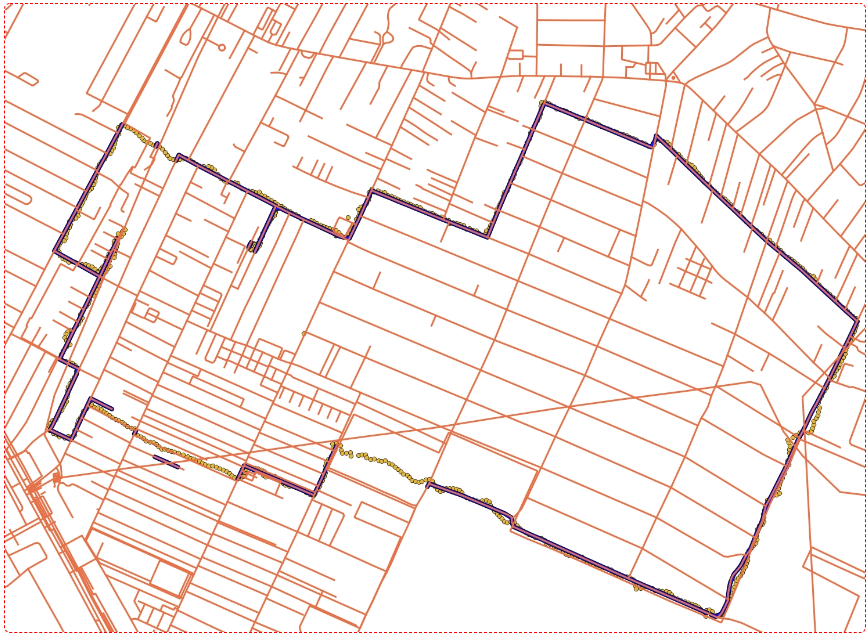
\includegraphics[max size={\textwidth}{\textheight}]{images/OSRM_map_matching_example.png}
    \end{column}
  \end{columns}
\end{frame}

\begin{frame}{What you need to deploy and use OSRM}
\begin{enumerate}
\item OSRM backend: based on Docker (cross-platform, but Linux is recommended)
\item OSRM frontend: I haven't used it before
\item (We will practice with OSRM in the next seminar)
\end{enumerate}
\end{frame}

\begin{frame}{Examples: Uber using OSRM}
\begin{enumerate}
\item Uber using OSRM to compute ETA
\item In Uber’s early days, we used a combination of routing engines to produce an ETA. (We didn’t have in-app navigation at this point, so we only used it for the ETA and map matching to display vehicle locations.)
\item \url{https://eng.uber.com/engineering-routing-engine/}
\end{enumerate}
\end{frame}

\begin{frame}{Examples: using OSRM to predict trip fare}
\begin{enumerate}
\item Kaggle competition of NYC taxi fare prediction
\item Intuition: using the driving distance predicted by OSRM will increase the model accuracy, better than Haversine distance
\item Result: adding this trip distance to the data led to 300/1500 on the leaderboard
\item \url{www.thinkdatascience.com/post/2020-03-03-osrm/osrm/}
\end{enumerate}
\end{frame}

\begin{frame}{Using OSRM in your projects}
\begin{enumerate}
\item Pre-processing noisy GPS data 
\item Travel mode choice: predicting the travel time/distance of different modes
\item Cycling route choice: simulate the influence of planned cycle infrastructure
\item https://eng.uber.com/engineering-routing-engine/
\end{enumerate}
\end{frame}

\section{Summary}
\begin{frame}{Summary}
\begin{enumerate}
\item OSRM is an open source routing software with multiple functions of routing/map matching.
\item It has the potential for many projects.
\item In the next seminar, we will practice with OSRM using Python.
\end{enumerate}
\end{frame}

\begin{frame}{Seminar outline}
\begin{enumerate}
\item 06/16: 路线规划的开源软件及应用(第一部分:软件介绍)
\item 06/23: 路线规划的开源软件及应用(第二部分:实践操作)
\item 06/30: 城市设施选址问题(第一部分:模型介绍)
\item 07/07: 城市设施选址问题(第二部分:开源软件)
\item 07/14: 城市设施选址问题(第三部分:案例分析)
\item 07/21: 选址-路线规划问题:无人机基站选址的案例
\end{enumerate}
\end{frame}

\end{document}
